\documentclass[titlepage,a4paper,12pt]{ltjsreport}

\usepackage{luatexja}
\usepackage{amsmath,amsfonts}
\usepackage{amsthm}
\usepackage{bm}
\usepackage[dvipdfmx]{graphicx}
\usepackage{color}
\usepackage{caption}
\usepackage{url}
\usepackage{listings}
\usepackage{abstract}
\usepackage{multicol}
\usepackage{geometry}
\usepackage{here}


\lstset{
    basicstyle={\ttfamily},
    identifierstyle={\small},
    commentstyle={\small},
    keywordstyle={\small\bfseries},
    ndkeywordstyle={\small},
    stringstyle={\small\ttfamily},
    frame={tb},
    breaklines=true,
    columns=fixed,
    basewidth=0.465em,
    numbers=left,
    numberstyle={\scriptsize},
    lineskip=-0.5ex
}


\begin{document}

\leftline{課題4 要求記述}
\rightline{256E0143
三留 慎太郎}

\begin{enumerate}
    \item 概要 \mbox{}\\
    対数正規分布の標準偏差を用いて、VS,S,M,L,VLの相対規模範囲を計算し、それぞれの中点を出力する。

    \item 詳細\mbox{}\\
    パーツ、パーツ規模、パーツごとのアイテム数、を用いてアイテムを単位とする。
    なお、パーツとアイテムが同じ、とみなす場合はパーツのアイテム数をすべて1として扱う

    相対規模範囲の計算は以下の手順に沿って行う

    \begin{enumerate}
        \item 部品規模を部品数で割り、部品ごとの規模を計算する。
        \item データを対数積変換するために、各サイズ値について自然対数InをとりIn($x_i$)を用いる。
        \item 対数正規変換した数値の平均$avg$を計算する。
        \item 平均を用いて分散$\sigma^2$を計算する。
        \item 分散の平方根である標準偏差$\sigma$を計算する。
        \item 対数区間を以下の対応で計算する。
        
        \begin{itemize}
            \item In(VS) = $avg - 2\sigma$
            \item In(S) = $avg - \sigma$
            \item In(M) = $avg$
            \item In(L) = $avg + \sigma$
            \item In(VL) = $avg + 2\sigma$
        \end{itemize}

        \item 自然対数値を対数計算して以下のように元の形に戻し、規模範囲の中点を求める。
        
        \begin{itemize}
            \item VS = $e^{In(VS)}$
            \item S = $e^{In(S)}$
            \item M = $e^{In(M)}$
            \item L = $e^{In(L)}$
            \item VL = $e^{In(VL)}$
        \end{itemize}

    \end{enumerate}


    \item 入力\mbox{}\\
    
    \begin{itemize}
        \item データの入力:csvファイル入力
        \item 入力ファイル:図\ref{data1},図\ref{data2}のように、カンマ区切りの表形式で表現し、パーツ名、パーツ規模、アイテム数を持つ。\\
        
        \begin{figure}[H]
            \centering
            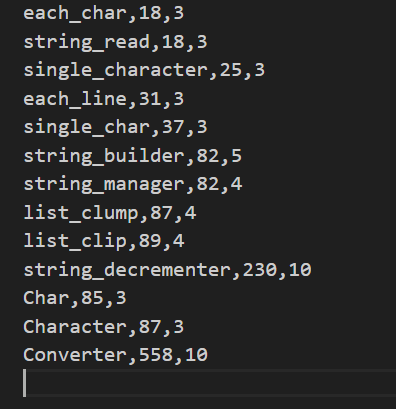
\includegraphics[width=0.4\textwidth]{../picture/課題4/4data1.png}
            \caption{規模データ}
            \label{data1}
        \end{figure}

        \begin{figure}[H]
            \centering
            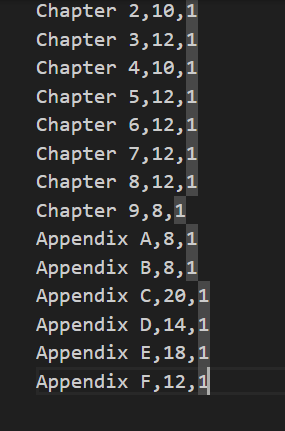
\includegraphics[width=0.4\textwidth]{../picture/課題4/4data2.png}
            \caption{パーツとアイテムが同じ場合の規模データ}
            \label{data2}
        \end{figure}
        
        \item 実行時の入力:コマンドラインに以下の形式で入力
         java プログラム名 実数値入力ファイル名
        \item 実行時入力例:java Program3 data\_program4\_1.csv\\
                

    \end{itemize}


    \item 出力\mbox{}\\
    \begin{itemize}
        \item 出力方法:コマンドライン出力
        \item 出力する値:VS,S,M,L,VLの相対規模範囲それぞれの中点。
        \item 精度:少数点以下第5位を四捨五入して表示する。
        \item 出力例:図\ref{kitaiti1}のように出力する値をそれぞれ改行して表示する。
        
        \begin{figure}[H]
            \centering
            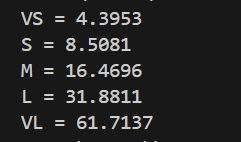
\includegraphics[width=0.4\textwidth]{../picture/課題4/kitaiti1.png}
            \caption{出力例}
            \label{kitaiti1}
        \end{figure}

    \end{itemize}


    \item テスト\mbox{}\\
    図\ref{testdata1},図\ref{testdata2}のデータをもちいてテストを行う。
    それぞれの期待値を図\ref{testkitaiti1},図\ref{testkitaiti2}に示す。\\

    \begin{figure}[H]
        \centering
        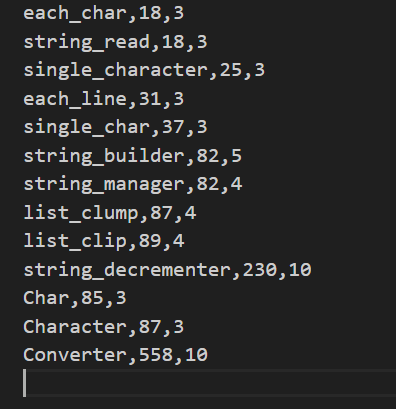
\includegraphics[width=0.4\textwidth]{../picture/課題4/4data1.png}
        \caption{プログラム規模データ}
        \label{testdata1}
    \end{figure}

    \begin{figure}[H]
        \centering
        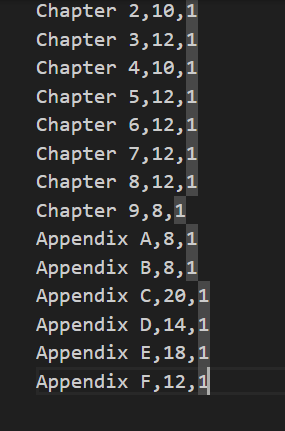
\includegraphics[width=0.4\textwidth]{../picture/課題4/4data2.png}
        \caption{文書規模データ}
        \label{testdata2}
    \end{figure}

    \begin{figure}[H]
        \centering
        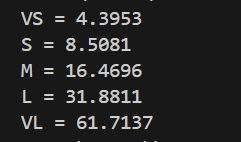
\includegraphics[width=0.4\textwidth]{../picture/課題4/kitaiti1copy.png}
        \caption{期待値1}
        \label{testkitaiti1}
    \end{figure}
    
    \begin{figure}[H]
        \centering
        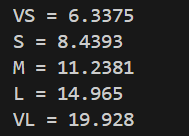
\includegraphics[width=0.4\textwidth]{../picture/課題4/kitaiti2.png}
        \caption{期待値2}
        \label{testkitaiti2}
    \end{figure}
    
     

\end{enumerate}



\end{document}